\addtolength{\tabcolsep}{-4.5pt}    
% \setlength{\mywidth}{0.1932\textwidth}
\bgroup
\def\arraystretch{0.5}%  1 is the default. Controls vertical spacing.
\begin{figure*}[]
\begin{tabular} {cc|cc|c}
 Label & Ground Truth & Pix2PixHD~\cite{wang2018pix2pixHD} &  SPADE~\cite{park2019SPADE} & Ours\\
% \includegraphics[width=0.1932\textwidth]{Images/Rec/Faces/label/28016.png} & \includegraphics[width=0.1932\textwidth]{Images/Rec/Faces/gt/28016.png} &
% \includegraphics[width=0.1932\textwidth]{Images/Rec/Faces/pix2pixhd/28016.png} &   \includegraphics[width=0.1932\textwidth]{Images/Rec/Faces/spade/28016.png} &  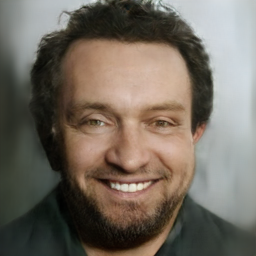
\includegraphics[width=0.1932\textwidth]{Images/Rec/Faces/ours/28016.png} \\

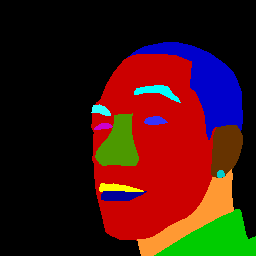
\includegraphics[width=0.1932\textwidth]{Images/Rec/Faces/label/28360.png} & 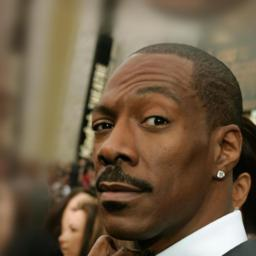
\includegraphics[width=0.1932\textwidth]{Images/Rec/Faces/gt/28360.jpg} &
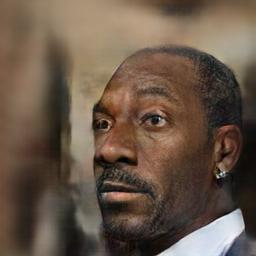
\includegraphics[width=0.1932\textwidth]{Images/Rec/Faces/pix2pixhd/28360.jpg}&jpg
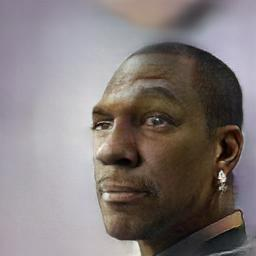
\includegraphics[width=0.1932\textwidth]{Images/Rec/Faces/spade/28360.jpg} &  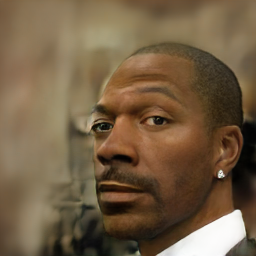
\includegraphics[width=0.1932\textwidth]{Images/Rec/Faces/ours/28360.png} \\

% 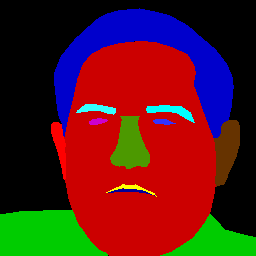
\includegraphics[width=0.1932\textwidth]{Images/Rec/Faces/label/28054.png} & \includegraphics[width=0.1932\textwidth]{Images/Rec/Faces/gt/28054.png} &
% \includegraphics[width=0.1932\textwidth]{Images/Rec/Faces/pix2pixhd/28054.png}&
% \includegraphics[width=0.1932\textwidth]{Images/Rec/Faces/spade/28054.png} &  \includegraphics[width=0.1932\textwidth]{Images/Rec/Faces/ours/28054.png} \\

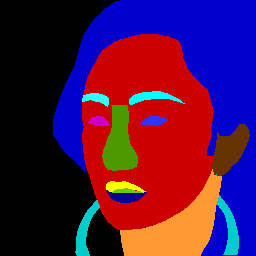
\includegraphics[width=0.1932\textwidth]{Images/Rec/Faces/label/28181.png} & 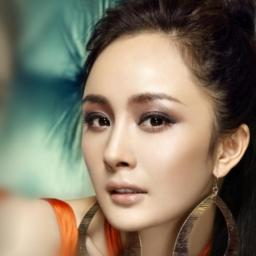
\includegraphics[width=0.1932\textwidth]{Images/Rec/Faces/gt/28181.jpg} &
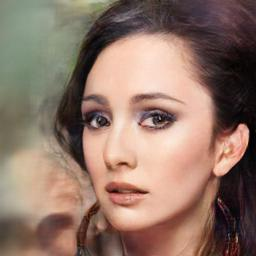
\includegraphics[width=0.1932\textwidth]{Images/Rec/Faces/pix2pixhd/28181.jpg}&
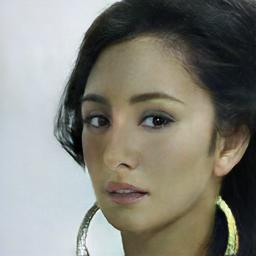
\includegraphics[width=0.1932\textwidth]{Images/Rec/Faces/spade/28181.jpg} &  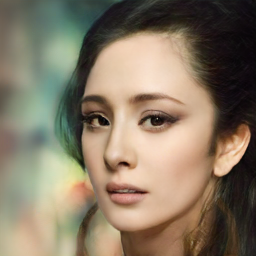
\includegraphics[width=0.1932\textwidth]{Images/Rec/Faces/ours/28181.png} \\

% \includegraphics[width=0.1932\textwidth]{Images/Rec/Faces/label/28434.png} & \includegraphics[width=0.1932\textwidth]{Images/Rec/Faces/gt/28434.png} &
% \includegraphics[width=0.1932\textwidth]{Images/Rec/Faces/pix2pixhd/28434.png}&
% \includegraphics[width=0.1932\textwidth]{Images/Rec/Faces/spade/28434.png} &  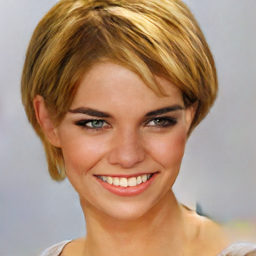
\includegraphics[width=0.1932\textwidth]{Images/Rec/Faces/ours/28434.png} \\

% \includegraphics[width=0.1932\textwidth]{Images/Rec/Faces/label/28059.png} & \includegraphics[width=0.1932\textwidth]{Images/Rec/Faces/gt/28059.png} &
% \includegraphics[width=0.1932\textwidth]{Images/Rec/Faces/pix2pixhd/28059.png}&
% \includegraphics[width=0.1932\textwidth]{Images/Rec/Faces/spade/28059.png} &  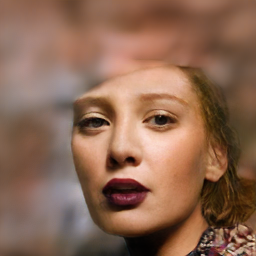
\includegraphics[width=0.1932\textwidth]{Images/Rec/Faces/ours/28059.png} \\


\end{tabular}
\vspace{-2mm}
	\caption{Visual  comparison  of  semantic  image  synthesis  results  on  the  CelebAMask-HQ dataset. We compare Pix2PixHD, SPADE, and our method.}
	\label{fig:CelebAMask-HQ results}	
\vspace{-3mm}	
 \end{figure*}
 \egroup
 \addtolength{\tabcolsep}{4.5pt}